\chapter{Supervised learning}
\section{Introductie}
In tegenstelling tot bij \emph{unsupervised learning} beschikken we bij \emph{supervised learning} over een dataset waarbij het gewenste resultaat al bijgevoegd is. Deze dataset wordt ook nog eens opgedeeld in twee delen: Een eerste deel waarmee het algoritme bijleert, en een tweede om de nauwkeurigheid van het algoritme te testen. Merk op dat indien de tweede dataset ook gebruikt zou worden om het algoritme te trainen, dit geen goed beeld zou geven van de werking. 

\paragraph{Voorbeeld}
Een eerste voorbeeld waarop dit mogelijk is, is een creditcardmaatschappij. Stel dat een nieuwe klant een aanvraag indient om een creditcard te krijgen. Dan moet het bedrijf verschillende parameters analyseren zoals de leeftijd, of de persoon getrouwd is, het loon, welke leningen er al aanwezig zijn, \dots Het resultaat van de aanvraag is dan binair: wordt de aanvraag aanvaard of niet? 

\paragraph{Voorbeeld}
Een tweede voorbeeld is in een ziekenhuis. Hierbij moet er opnieuw aan de hand van een aantal parameters beslist worden of een pati\"ent opgenomen moet worden op intensive care. Aangezien dit een duur proces is, wensen ziekenhuizen dit enkel te doen voor pati\"enten met een hoog risico.

Algemeen heeft met dus een probleem met een aantal (discrete) uitkomsten. Hiervoor ontwikkelen we een oplossing waarbij een functie getraind wordt met een bestaande dataset. Dit wordt ook vaak \emph{classification} of \emph{inductive learning} genoemd.
\section{Voorbeeld en terminologie}
De data wordt gedefinieerd als een set van $k$ attributen: ${A_1, A_2,..,A_k}$. Elke rij heeft ook een label met een reeds gedefinieerde klasse. Hiervan komt de naam \emph{supervised}, we beschikken over leermateriaal. Het doel is om deze gegevens te gebruiken om een model zo te trainen dat een toekomstige rij, waarbij alle attributen aanwezig zijn, een correct label toe te kennen.
Na de training kan de data getest worden op een tweede dataset. Deze dataset bestaat uit een aantal rijen waarvan de klasse reeds bekend is. Met kan de \emph{accuracy} van het model dan als volgt berekenen:

\begin{equation}
\textrm{Correctheid} = \frac{\textrm{juiste gevallen}}{\textrm{totaal aantal testcases}}
\end{equation}

Algemeen volgen we dus dit patroon:

\begin{equation}
\textrm{Training data} \rightarrow \textrm{Learning  algoritm} \rightarrow \textrm{Model} \rightarrow \textrm{Test data} \rightarrow \textrm{Accuracy}
\end{equation}

Het is belangrijk om zich het doel te blijven herinneren tijdens dit proces. Stel in het voorbeeld van het creditcardmaatschappij dat we gewoon steeds \emph{geaccepteerd}  antwoorden. Dan zullen we dus een \emph{accuracy} van 50\% hebben. Het doel van het supervised learning algoritme is dus om (veel) beter te doen dan de reeds gebruikte methode.

Het aanleren wordt dus als volgt gedefinieerd. Stel dat we een dataset \emph{D} hebben met een taak \emph{T} en een manier om de kwaliteit te meten \emph{M}. Een computersysteem leert dan van \emph{D} om taak \emph{T} uit te voeren, indien na het leren het systeem beter presteert als het taak \emph{T} uitvoert. Dit wordt gemeten via \emph{M}.

Er is dus een cruciaal concept waar we steeds rekening mee moeten houden indien we gebruik maken van \emph{supervised learning}: De test- en trainingsdata moet voldoende representatief zijn voor de data die men in het echt zal krijgen.
\section{Decision trees}
Een eerste, simpele maar toch effici\"ente vorm van supervised learning zijn \emph{decision trees}. Deze beslissingsbomen werken volgens een simpel principe. Bovenaan de boom staat een eerste attribuut. Vanuit deze knoop vertrekken verbindingen naar andere knopen. Elke verbinding stelt een waarde van het attribuut voor.

\begin{figure}[h]
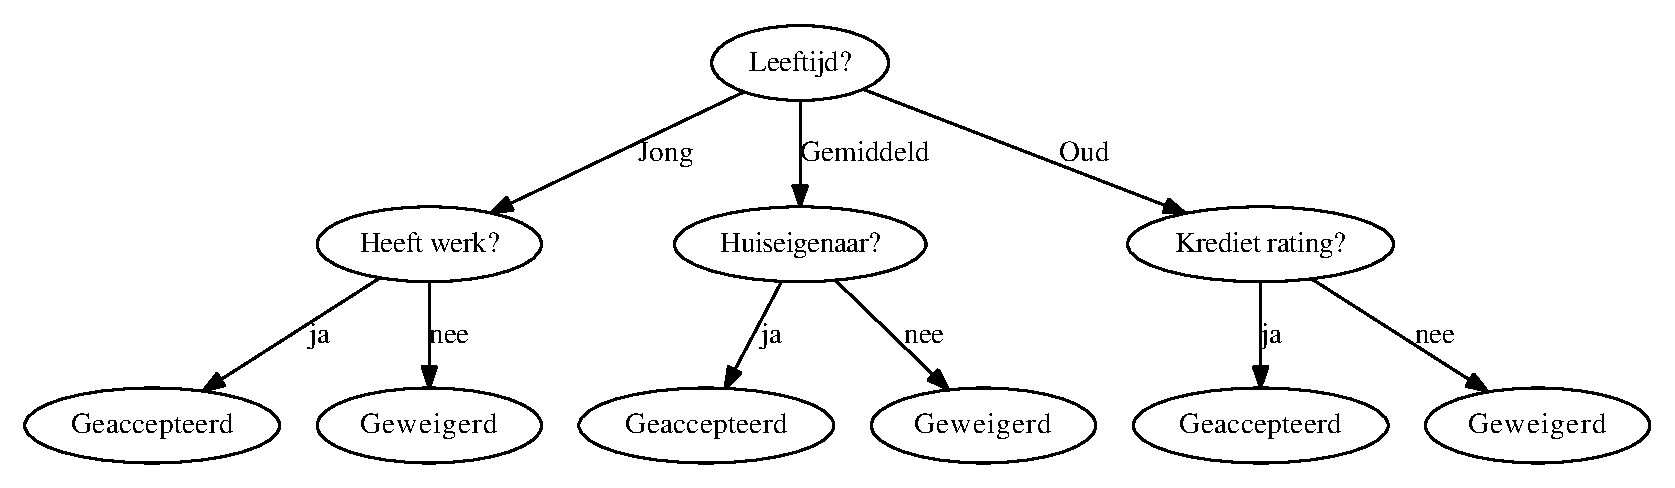
\includegraphics[width=\textwidth]{res/1}
\caption{Een voorbeeld van een beslissingsboom voor een creditcardmaatschappij.}
\label{fig:vb1_dt}
\end{figure}

Deze boom is afhankelijk van de gegeven data en is niet uniek, noch optimaal. Er bestaat een kleinere boom die dezelfde info geeft in minder nodes. We moeten dus proberen een zo klein mogelijk boom te construeren. Dit is echter geen triviale opgave en alle huidige algoritmes geven een benadering.

De boom kan worden omgezet naar een serie regels. Elk pad van de beginknoop tot aan een blad is een regel. Voor figuur ~\ref{fig:vb1_dt} geeft dit dus volgende regels:
\begin{itemize}
\item Leeftijd = jong, heeft werk? = ja $\Rightarrow$ Class = Geaccepteerd
\item Leeftijd = jong, heeft werk? = nee $\Rightarrow$ Class = Geweigerd
\item ...
\end{itemize}
Elk van deze regels heeft dan ook een \emph{support} en \emph{confidence} afhankelijk van de gebruikte dataset.

\subsection{Een simpel algoritme}
Een mogelijk algoritme is een \emph{divide-and-conquer} algoritme. 
%%%%%%%%%%%%%%%%%%
% Indien dit gekopieerd wordt, zie: https://en.wikibooks.org/wiki/LaTeX/Algorithms
%%%%%%%%%%%%%%%%%%
\begin{algorithm}
\caption{Voorbeeld van een beslissingsboom constructie algoritme}
\begin{algorithmic}[1]
\Require D: Training data, A: Attributen, T: Een knoop van de boom, C: De verzameling van klassen
\Function{maakBeslissingsBoom}{D,A,T}
\If {$D$ bevat enkel data van een bepaalde klasse $c_j \in C $}
    \State maak $T$ een blad met klasse $c_j$;
\ElsIf{ $A = \emptyset$ }
	\State Maak van $T$ een blad met het label van klasse $c_j$,
    \State waarbij $c_j$ de meest voorkomende klasse in $D$ is.;
\Else
	\State // $D$ bevat een mix van klassen.We selecteren een 
	\State // attribuut om $D$ verder te verdelen in subsets 
	\State // zodat elke subset minder onzuiverheden bevat.
    \State $p_0 = $ puriteitEval($D$)
    \For{ $A_i \in \{A_1, A_2, ..., A_k\} $ }
    	\State $p_i$ = puriteitsEval($A_i,D$); 
    \EndFor
    \State Selecteer $A_g \in \{A_1, A_2, ..., A_k\} $ met de minste puurheid,
    \State berekend met $p_0 - p_i$;
    \If{ $p_0 - p_g < drempelwaarde$ }
    	\State Maak van $T$ een blad met label $c_j$;
    \Else
    	\State Maak van T een beslissingsknoop voor $A_g$;
		\State Verdeel $D$ dan in $m$ sets $D_1, D_2, ..., D_m$ gebaseerd op 
        \State $A_g$, met de mogelijke waarden: $\{v_1,v_2,..v_m\}$ 
        \For{ $D_j$ in $\{D_1,D_2,..D_m\}$ }
        	\If{ $D_j \neq \emptyset $ }
            	\State Maak een tak $T_j$ voor $v_j$ als kind van $T$.
                \State decisionTree( $D_j, A-\{A_g\}, T_j$ )
            \EndIf
        \EndFor
    \EndIf
\EndIf
\EndFunction
\end{algorithmic}
\end{algorithm}

Bij dit algoritme nemen we aan dat alle data categorisch is. De boom wordt op een \emph{top-down} recursieve manier opgesteld. Dit wil zeggen dat we beginnen bij de bovenste knoop van de boom en zo verder afdalen tot de bladen gevormd zijn. Elementen uit de dataset worden verder onderverdeeld gebaseerd op hun attributen.

Het bovenste algoritme heeft enkele voorwaarden op te stoppen:

\begin{itemize}
\item Indien er geen elementen meer over zijn
\item Er zijn geen attributen meer die onderverdeeld moeten worden
\item Alle elementen bij een knoop behoren tot dezelfde klasse
\end{itemize}

De sleutel tot succes bij dit algoritme is de keuze van het attribuut om een tak te maken. Het doel is om de data zo puur mogelijk te maken: Een subset van data wordt als puur aanzien indien alle data tot dezelfde klasse behoort. Voor we verder ingaan op het maken van deze keuze moeten we eerst begrijpen wat puurheid nu eigenlijk is. We verklaren dit aan de hand van \emph{informatietheorie}.

\subsection{Informatietheorie}
Informatietheorie is een onderdeel van de wiskunde dat zich bezig houdt de opslag en verwerking van informatie. Het levert ons een basis om de inhoud van data te beschrijven. Een manier om dit beter te begrijpen is om dit voor te stellen als een antwoord op een vraag: Zal mijn worp kop of munt zijn? Indien men op voorhand al info heeft, men weet bijvoorbeeld dat de munt vervalst is, dan is het antwoord op de vraag minder relevant. Indien men dit nog niet weet, dan zou extra kennis dus welkom zijn. Het antwoord heeft dus een grotere waarde.

Informatietheorie gebruikt ditzelfde concept, maar gebruikt geen geld om de waarde van informatie uit te drukken, maar \emph{bits}. Een bit is net genoeg info om het antwoord te geven op een ja/neen vraag waarover men geen idee heeft, zoals het opwerpen van een munt.

Een belangrijke manier om hoeveelheden informatie uit te drukken is entropie. Entropie is een maat voor informatiedichtheid in een reeks gebeurtenissen. Deze entropie wordt gedefinieerd als:
\begin{equation}
E(p) = - \sum_{i=1}^{n} p_i \log_{2}{p_i} [bit]
\end{equation}
Waarbij $p_i$ een kans is op de uitkomst van $u_i$ bij experiment $A$. Of in het geval van beslissingsbomen: De kans op klasse $c_j$ in data set $D$. We kunnen deze entropie gebruiken als een maat voor de puurheid van een dataset $D$. Een voorbeeld: Stel dat een dataset bestaat uit een lijst van positieve en negatieve tweets over een bepaald onderwerp.
\begin{enumerate}
\item Een dataset $D$ heeft 50\% positieve tweets en 50\% negatieve. De entropie is dan: $E(D) = -0,5\cdot \log_2{0,5} - 0,5\cdot \log_{2}{0,5} = 1 bits$
\item Een dataset $D$ heeft 20\% positieve tweets en 80\% negatieve. De entropie is dan: $E(D) = -0,2\cdot \log_2{0,2} - 0.8\cdot \log_{2}{0,8} = 0,722 bits$
\item Een dataset $D$ heeft 100\% positieve tweets en 0\% negatieve. De entropie is dan: $E(D) = -1\cdot \log_2{1} - 0\cdot \log_{2}{0} = 0 bits$
\end{enumerate}

Hieruit volgt dat naarmate de data puurder wordt, de entropie steeds kleiner wordt. We kunnen deze eigenschap gebruiken voor het opstellen van beslissingsbomen.

De toename van informatie en afname van entropie is dan het verschil tussen de entropie voor een tak wordt toegevoegd en de entropie erna. Deze toename wordt in de literatuur vaak \emph{information gain} genoemd.

Stel nu dat we een attribuut $A_i$ met $v$ mogelijke waarden hebben en deze attribuut de wortel van de huidige boom maken, dan zal dit de dataset $D$ onderverdelen in $v$ subsets $D_1, D_2, ...$. De entropie wordt dan:
\begin{equation}
E_{A_i}(D) = \sum_{j=1}^{v} \frac{|{D_j}|}{|D|} \cdot E(D_j)
\end{equation}

Een concreet voorbeeld bij het opstellen van een beslissingsboom voor een creditcardmaatschappij met volgende data:
\begin{table}[h]
\centering
\caption{Een verzameling met applicaties $D$.}
\label{tabel:sl_ex1}
\begin{tabular}{c|c|c|c|c|c}
  \textbf{ID} & \textbf{Leeftijd} & \textbf{Heeft werk} & \textbf{Huiseig.} & \textbf{Credit rating} & \textbf{Klasse} \\
1 & jong 	& neen 	& neen 	& redelijk & neen  \\
2 & jong 	& neen 	& neen 	& goed & neen  \\
3 & jong 	& ja 	& neen 	& goed & ja  \\
4 & jong 	& ja 	& ja 	& redelijk & ja \\
5 & jong 	& neen 	& neen 	& redelijk & neen \\
6 & gem. & neen & neen & redelijk & neen \\
7 & gem. & neen & neen & goed & neen \\
8 & gem. & ja 	& ja 	& goed & ja \\
9 & gem. & neen & ja 	& excellent & ja \\
10 & gem. & neen & ja 	& excellent & ja \\
11 & oud 	& neen 	& ja 	& excellent & ja \\
12 & oud 	& neen 	& ja 	& goed & ja \\
13 & oud 	& ja 	& neen 	& goed & ja \\
14 & oud 	& ja 	& neen 	& excellent & ja \\
15 & oud 	& neen 	& neen 	& redelijk & neen \\
\end{tabular}
\end{table}

De entropie van deze totale dataset wordt berekend a.d.h.v. de klasse:
\begin{equation}
E(D) = -\frac{6}{15} \cdot \log_2 \frac{6}{15} - \frac{9}{15} \cdot \log_2 \frac{9}{15} = 0.971
\end{equation}

Vervolgens berekenen we per attribuut de entropie en de winst in informatie indien dit attribuut de wortel van de beslissingsboom zou zijn.

\begin{equation}
E_{leeftijd}(D) = \frac{5}{15} \cdot E(D_1) + \frac{5}{15} \cdot E(D_2) + \frac{5}{15} \cdot E(D_3)  
\end{equation}
Met:
\begin{equation}
E(D_1) = -\frac{3}{5} \cdot \log_2 \frac{3}{5} - \frac{2}{5} \cdot \log_2 \frac{2}{5} = 0.971
\end{equation}
\begin{equation}
E(D_2) = -\frac{3}{5} \cdot \log_2 \frac{3}{5} - \frac{2}{5} \cdot \log_2 \frac{2}{5} = 0.971
\end{equation}
\begin{equation}
E(D_3) = -\frac{4}{5} \cdot \log_2 \frac{4}{5} - \frac{1}{5} \cdot \log_2 \frac{1}{5} = 0.722
\end{equation}
Levert dit:
\begin{equation}
E_{leeftijd}(D) = \frac{5}{15} \cdot 0.971 + \frac{5}{15} \cdot 0.971 + \frac{5}{15} \cdot 0.722 = 0.888
\end{equation}
Met als informatiewinst:
\begin{equation}
winst(D,leeftijd) = 0.971 - 0.888 = 0.083
\end{equation}
Zo kunnen we voor elk attribuut de winst berekenen. Dit levert voor de attributen \emph{Heeft werk}, \emph{Huiseigenaar}, \emph{Krediet rating}:
\begin{equation}
winst(D,Heeft\ werk) = 0.9721 -  0.647 = 0.324
\end{equation}
\begin{equation}
winst(D,Huiseigenaar) = 0.9721 -  0.551 = 0.420
\end{equation}
\begin{equation}
winst(D,Krediet rating) = 0.9721 - 0.608 = 0.363
\end{equation}

We kiezen het attribuut met de grootste winst aan informatie, in dit geval \emph{Huiseigenaar} als wortel van onze boom. Deze ziet er dan zo uit:

\begin{figure}[h]
\centering
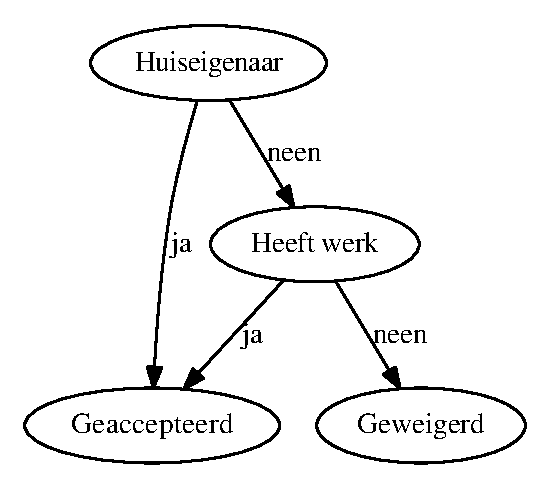
\includegraphics[width=0.6\textwidth]{res/ch5_dt_vb2.eps}
\caption{De beslissingsboom opgesteld door het algoritme}
\end{figure}

Tot nu toe zijn we ervan uitgegaan dat attributen discreet zijn. Het algoritme werkt echter ook met continue attributen. Dit kunnen we doen door met intervallen te werken. Het moeilijke hierbij is de keuze van de waarde die dient als onderverdeling van deze intervallen. Hiervoor gebruiken we opnieuw de informatiewinst. We sorteren eerst de waarden in onze dataset in toenemende volgorde: $\{v_1,v_2,...v_k\}$. Een van de mogelijke waarden voor de drempel is dan deze tussen $v_i$ en $v_{i+1}$. We proberen alle drempels en kiezen degene die de maximale winst oplevert. Het probleem bij deze aanpak is dat men zo kan blijven onderverdelen aangezien de waarden continu zijn.

Een laatste probleem bij het opstellen van beslissingsbomen is \emph{overfitting}. Hierbij is de boom teveel aangepast aan de trainingdata en niet genoeg aan het algemene geval. De symptomen hiervan zijn vaak duidelijk omdat de boom diep is en enorm veel takken bevat. Dit is vaak te wijten aan ruis of andere afwijkingen. Er zijn twee manieren om dit te vermijden:
\begin{enumerate}
\item Bij \emph{pre-pruning} wordt de constructie van de boom vroegtijdig gestart. De moeilijkheid hierbij is om te weten wanneer men moet stoppen.
\item Bij \emph{post-pruning} worden takken verwijderd van een reeds gemaakte boom gebaseerd op een statisch model dat de fouten per tak berekent.
\end{enumerate}

\section{K-nearest neighbour}
Een tweede algoritme voor \emph{supervised learning} dat we zullen bespreken is het \emph{K-nearest neighbour} algoritme. In tegenstelling tot bijvoorbeeld beslissingsbomen bouwt KNN geen model van de training data.

Algoritme \ref{algo:knn} beschrijft hoe dit gebruikt wordt in R en het resultaat van dit script is figuur \ref{figure:knn_after}.

\begin{algorithm}
\caption{Het kNN algoritme}
\label{algo:knn}
\begin{algorithmic}[1]
\Require D: Training data, d: het element dat geclassificeerd moet worden, k: Het aantal buren.
\Function{kNN}{D,d,k}
	\State bereken\_afstand($d,D$);
    \State $P$ = kies\_k\_dichtste($D$,k);
    \State d->klasse = meest\_frequente($P$);
\EndFunction
\end{algorithmic}
\end{algorithm}
Hierbij geven we $d$ dus een klasse door eerst alle afstanden in $D$ tot aan $d$ te berekenen. Hieruit kiezen we dan $k$ punten die we in de verzameling $P$ plaatsten. De klasse van $d$ stellen we dan gelijk aan de meest voorkomende klasse in $P$. We gaan er dus van uit dat de kans op klasse $c_j$, indien we $n$ kennen, gelijk is aan $\frac{n}{k}$.

\begin{equation}
p(c_j|d) = \frac{n}{k}
\end{equation}

Cruciaal hierbij is de keuze van de afstandsberekening. Het meest voor de hand liggende is natuurlijk de euclidische afstand, maar alternatieven---zoals de \emph{Manhattan distance}---zijn ook mogelijk. De keuze is vaak afhankelijk van de applicatie.

\emph{k} is meestal empirisch gekozen door handmatig te kiezen of via een controle set.

\begin{figure}[h]
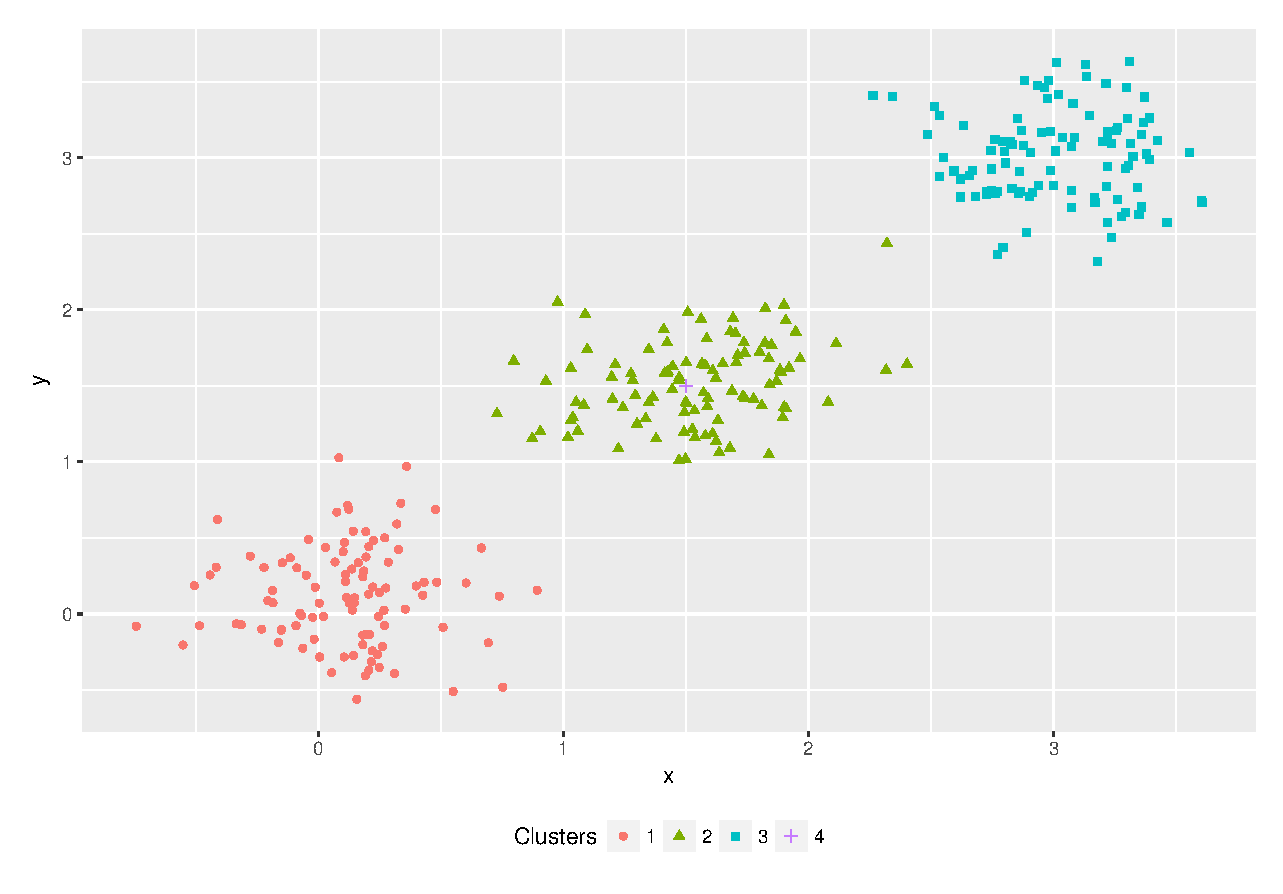
\includegraphics[width=\textwidth]{res/knn_before.eps}
\caption{De data voor het knn algoritme wordt toegepast.}
\label{figure:data-knn}
\end{figure}

\newpage
\paragraph{Voorbeeld} We maken gebruik van de \emph{package} FNN. Stel dat we reeds geclassificeerde data hebben, welke in figuur \ref{figure:data-knn} gevisualiseerd is. In de figuur zijn er 3 groepen met elk een klasse en 1 testpunt. De code om het punt te classificeren ziet er als volgt uit:

\inputminted{R}{code/knn.R}

\begin{figure}[h]
\includegraphics[width=\textwidth]{res/knn_after.eps}
\caption{De data nadat het KNN algoritme wordt toegepast: het punt behoord tot de juiste klasse.}
\label{figure:knn_after}
\end{figure}

\subsection{Bemerkingen bij KNN}
Het KNN algoritme heeft enkele voordelen:
\begin{itemize}
\item De eenvoudigheid. KNN is een zeer eenvoudig algoritme om te begrijpen en implementeren. Desondanks heeft KNN al heel wat goede resultaten opgeleverd.
\item KNN kan overweg met complexe grenzen tussen data.
\end{itemize}
Er zijn echter ook enkele nadelen aan verbonden.
\begin{itemize}
\item In tegenstelling tot bijvoorbeeld beslissingsbomen levert KNN geen begrijpbaar model op.
\item Omdat er geen model wordt gemaakt en de classificatie meteen gebeurt, is KNN traag tijdens deze classificatie.
\end{itemize}

\subsection{Besluit}
\emph{Supervised learning} is een reeks van technieken die reeds geclassificeerde data gebruikt om toekomstige classificaties te voorspellen. Twee van deze technieken hebben we besproken in deze cursus. Bij de eerste, beslissingsbomen, wordt er een boomstructuur opgesteld a.d.h.v. de trainingsdata waarna de testdata eenvoudig geclassificeerd kan worden. Bij de tweede techniek, KNN, krijgen we geen verstaanbaar model maar deze techniek werkt wel voor complexe data.